\clearpage

\section{Theorie}
\label{theorie}

\subsection{Mobilfunkstandards}

\subsection{SIM-Karten}

\subsection{Authentifizierungsvorgang}
\label{authentifizierungsvorgang}

\subsection{Milenage Algorithmus}
\label{milenage}
Zwischen \ac{SIM}-Karte und Netzprovider muss eine sichere Authentifizierung und Kommunikation gewährleistet werden können. Dies war wie in Kapitel \Verweis{geschichte-usim} bereits beschrieben mit dem ersten entwickelten Algorithmus des \ac{3GPP} nicht mehr gewährleistet, weshalb mit der Entwicklung des neuen Netzstandards auch ein neuer Algorithmus entwickelt wurde, namentlich der Milenage Algorithmus. \\
Dieser verfügt über die sieben Funktionen \emph{f1}, \emph{f1*}, \emph{f2}, \emph{f3}, \emph{f4}, \emph{f5}, \emph{f5*} mit Hilfe derer eine sichere Authentifizierung und Schlüsselgenerierung ermöglicht wird. Die Funktionen mit \emph{*} sind dabei lediglich für die Re-synchonisation nötig. \\
3GPP hat, wie auch beim Vorgänger, diese Funktionen nicht näher spezifiziert und ermöglicht den Netzprovidern eigenen Lösungen zu implementieren. Stattdessen wird beschrieben in welchem Kontext diese Funktionen Anwendung finden und definieren generelle Anforderungen an diese Algorithmen \cite{3gpp.35.205}.

Der Milenage Algorithmus hat wie erwähnt zwei Hauptaufgaben, nämlich einerseits die Authentifizierung, als auch die Generierung eines Schlüssel, um die versendeten Nachrichten zu ver- und entschlüsseln. Wenn es um die Authentifizierung geht muss sich einerseits die SIM-Karte, bzw. das \ac{UE}, gegenüber dem Netzprovider authentifizieren, aber andererseits muss sich auch das Netzwerk gegenüber der SIM-Karte authentifizieren. Damit soll die Möglichkeit der Man-in-the-Middle Attacken reduziert werden, die es einem Außenstehenden erlauben die Kommunikation mitzulesen. Auch so genannte Replay-Attacken, bei denen zuvor aufgezeichnete Daten genutzt werden, sind nicht möglich, auf Grund der \acl{SQN} \cite{spitz11}.

In den nachfolgenden Unterkapiteln werden die Vorteile und die Funktionsweise des Algorithmus, sowie die Funktionsweise der eingesetzten Blockschiffrierung \ac{AES} erläutert.

 \subsubsection{Warum Milenage sicher ist}
 In Kapitel \Verweis{authentifizierungsvorgang} wurde schon erklärt, dass das die Mechanismen zur Authentifizierung und zum Schlüsselaustausch angepasst wurden und durch einige Änderungen Vorteile mit sich bringen, aber auch der weiterentwickelte Algorithmus zur Berechnung der Daten weißt einige Vorteile auf. \\
 Ein wichtiger Punkt dabei ist, dass der Vorgänger geheim war und Milenage nicht, denn ein solcher Algorithmus sollte öffentlich sein, damit möglichst viele Leute drüber gucken können und eventuelle Schwachstellen rechtzeitig bemerkt werden. 
 
 Stephan Spitz zeigt in seinem Buch ``Kryptographie und IT-Sicherheit''  \cite{spitz11} drei wesentliche Gründe auf, die den Algorithmus sicher machen:
 
 \paragraph{Ergebnisse mit hoher Entropie}
 Wenn der Schlüssel \ac{K} unbekannt ist und die die Eingabeparameter \ac{SQN}, \ac{RAND} und \ac{AMF} variieren, dann werden ``sehr gute Pseudo-Zufalls-Ergebnisse mit einer hohen Entropie'' \cite{spitz11} erreicht. Dafür muss aber auch eine gute Blockschiffrierung wie AES eingesetzt werden.
 
 \paragraph{Keine Rückschlüsse auf K möglich}
 Wenn die Eingabe- und Ausgabeparameter der einzelnen Funktionen \emph{f1} bis \emph{f5} analysiert werden, lassen sich keine Rückschlüsse auf den Schlüssel K oder das \acf{OP} ziehen, auch nicht auf Teile dessen. Dies hängt unter anderem damit zusammen, dass K nicht direkt in die Funktionen eingeht.
 
 \paragraph{Schlüssellänge}
 Brut-Force-Angriffe, also stumpfes ausprobieren der Schlüssel, ist auf Grund der Schlüssellänge von 128 Bits zu aufwändig mit aktuellen Rechnern.
 
 \textbf{Kapitel über die Vorraussetzungen an einzelne Parameter, bzw. wie diese angepasst werden können?}

 \subsubsection{Funktionsweise}
 In Kapitel \Verweis{authentifizierungsvorgang} wurde beschrieben, welche Daten zwischen \ac{AuC} und \ac{UE} verschickt werden, jedoch nicht wie diese Daten generiert werden. Es gibt einige Werte, die auf der \ac{USIM} und der Datenbank des \ac{AuC} fest eingespeichert sind. Diese sind der \ac{OP} und \ac{K}, sowie jeweils fünf Rotations- und XOR-Konstanten (r1, ..., r5 und c1, ... c5). Welche Funktion welche Werte benötigt und generiert zeigt dabei \Abbildung{funktionsubersicht}.
 
 \begin{figure}[htp]
  \begin{center}
   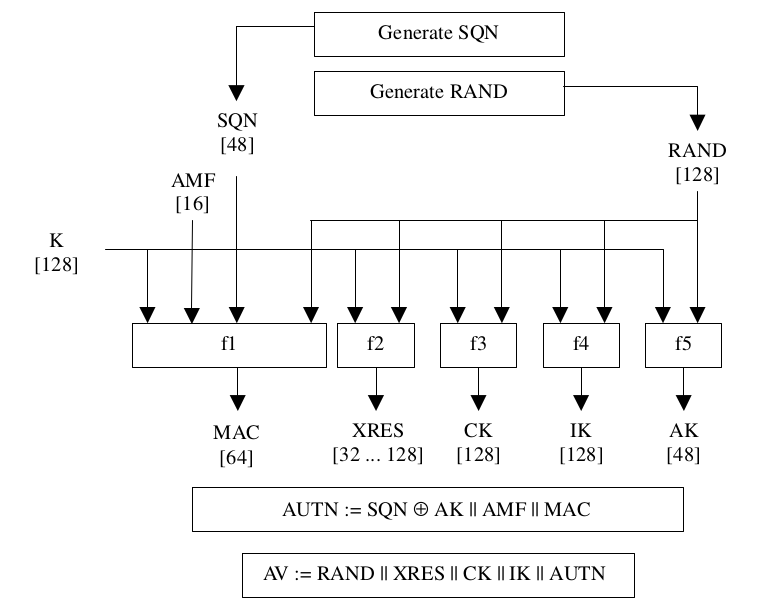
\includegraphics[width=300pt]{generation_of_authentication_vectors}
  \end{center}
  \caption{Übersicht über die Generierung der Authentifizierungsvektoren \cite{3gpp.33.102}}
  \label{fig:funktionsubersicht}
 \end{figure}
 
 In \Abbildung{funktionsubersicht} ist zu sehen, dass zu Beginn die \ac{SQN} generiert wird. Diese ist insgesamt 48 Bits lang und besteht aus den beiden Teilen SEQ und IND, mit SEQ als der die eigentliche Sequenznummer und IND als Arrayindex. Dieser Index wird benötigt, da auf der SIM-Karte sind die letzten SQNs in einem Array gespeichert. Die empfohlene Arraygröße ist 32, was für IND eine Länge von fünf Bits bedeutet. Mit diesem Index kann nachher die Aktualität der SEQ überprüft werden.\cite{3gpp.33.102} \\
 Für die Bildung der SEQ selbst gibt es drei verschiedene Möglichkeiten:
 \begin{itemize}
  \item teilweise zeitbasiert
  \item nicht zeitbasiert
  \item komplett zeitbasiert
 \end{itemize}
 
 Die einfachste Variante ist die nicht zeitbasierte Lösung, bei der lediglich ein Zähler hochgezählt wird mit jeder Authentifizierungsanfrage. Die SEQ ist initial also 0 und wird hochgezählt und gleichzeitig vom \ac{AuC} in einer Datenbank gespeichert \cite{3gpp.33.102}. Auf die anderen Möglichkeiten wird hier nicht näher eingegangen, da sie in dieser Arbeit keine Anwendung fanden.
 
 Als nächstes wird die \ac{RAND} gebildet. Das Verfahren, wie der Netzprovider diese RAND generiert darf nicht offen gelegt werden, da dies die Sicherheit stark beeinflussen würde. Generell handelt es sich dabei um eine 128-bit lange Zufallszahl, die für jede Funktion benötigt wird.
 
 \Abbildung{funktionsubersicht} zeigt zwar, welche Variablen in die Funktionen einfließen und welche Werte sie zurückgeben, aber sie zeigt nicht näher wie diese Werte nun verarbeitet werden. Dies zeigt \Abbildung{schematisch_milenage} besser. Dort ist zu erkennen, dass \emph{f2} bis \emph{f5*} nach dem selben Schema berechnet werden können und \emph{f1}, sowie \emph{f1*} noch einige zusätzliche Parameter haben.
 
 Zunächst die Erklärung der Symbole sowie einiger weiterer Abkürzungen. \ac{OPc} wird durch folgende Formel generiert:
 \begin{center}
  $OP_{C} = OP \oplus E(OP)_{K}$
 \end{center}
 
 $E()$ ist die Blockschiffrierung. In diesem Falle wird also \ac{OP} mit dem Schlüssel \ac{K} verschlüsselt. Welche Verschlüsselung gewählt wird, wird von 3GPP nicht vorgegeben. In dieser Arbeit wurde \ac{AES} verwendet, welche im Kapitel \Verweis{aes} näher beschrieben wird. \\
 Der verschlüsselte OP wird dann im zweiten Schritt über XOR ($\oplus$) mit dem ursprünglichen OP verknüpft.
 
 \begin{figure}[ht]
  \begin{center}
   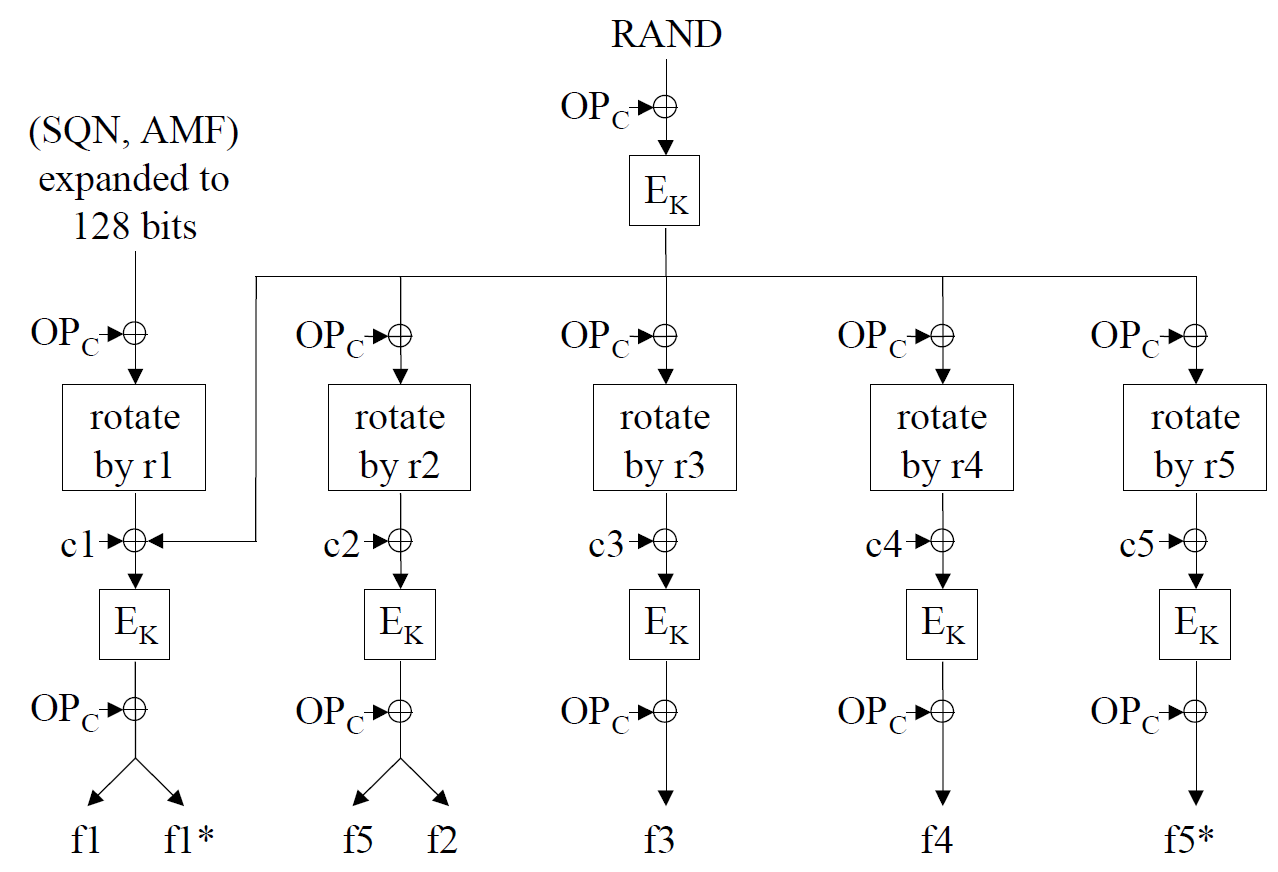
\includegraphics[width=400pt]{detailed_generation_of_authentication_vectors}
  \end{center}
  \caption{Schematische Darstellung zur Berechnung der Authentifizierungsvektoren \cite{3gpp.33.102}}
  \label{fig:schematisch_milenage}
 \end{figure}
 
 In \Abbildung{schematisch_milenage} ist weiterhin der Funktionsblock ``rotate by r'' zu lesen. Beim rotieren wird der Eingabewert um die Anzahl an Bits des Wertes von r rechts rotiert und die Bits die herausfallen links wieder eingefügt. Beispielsweise wird aus 110101 bei einem Rotationswert r von 2: 011101.
 
 Mit den genannten Infos ist verständlich, dass die Funktionen \emph{f2} bis \emph{f5*} ausgehen von einem verschlüsselten $RAND \oplus OP_{C}$, welcher in der Dokumentation auch als TEMP bezeichnet wird. Dieser Wert wieder wieder über XOR-mit $OP_ {C}$ verknüpft und um die entsprechende Rotationskonstante r rotiert. Im Anschluss wieder eine XOR-Verknüpfung mit der speziellen XOR-Konstante c und die Schiffrierung des Ausgabewertes. Im letzten Schritt wird dieser dann nochmal über XOR mit $OP_{C}$ verknüpft. \\
 Wie die \Abbildung{schematisch_milenage} zeigt funktionieren \emph{f1} und {f1*} sehr ähnlich. Bevor jedoch TEMP in die Berechnung einfließt wird SQN und AMF auf 128 Bits erweitert und bekommt in der Dokumentation die Bezeichnung IN1. IN1 besteht aus SQN und AMF abwechselnd konkateniert, also SQN $\|$ AMF $\|$ SQN $\|$ AMF. \cite{3gpp.33.102}
 
 
\subsection{AES / Rijndael}
\label{aes}
 Rijndael oder \ac{AES} sind beide Blockverschlüsselungen. Das bedeutet, dass der zu verschlüsselnde Text in gleich große Blöcke aufgeteilt wird und jeder Block mit einem Schlüssel chiffriert wird. Die Blocklänge des verschlüsselten Text bleibt dabei gleich. \\
 Der Unterschied zwischen Rijndael und AES besteht lediglich in der Länge der Text- uns Schlüsselblöcke und ist sonst identisch. Für Rijndael gilt, dass Block- und Schlüssellänge unabhängig von einander auf Vielfache von 32 Bits definiert werden können. Minimal müssen beide aber 128 Bits lang sein und maximal 256 Bits \cite{daemon02}. \\
 AES auf der anderen Seite hat die Blocklänge auf 128 Bits festegelegt und die Schlüssellänge darf nur 128, 192 oder 256 Bits betragen \cite{AES-FIPS}.
 
 Im folgenden soll kurz die Geschichte von AES beziehungsweise Rijndael erläutert werden und wie der Verschlüsselungsalgorithmus der beiden funktioniert.
 
 \subsubsection{Geschichte}
 \label{aes-geschichte}
 
 
 \subsubsection{Funktionsweise}
 \label{aes-funktion}
 
 \cite{paar09}
 
 \clearpage

\subsection{PPP}
Zur Bereitstellung einer Punkt-zu-Punkt-Verbindung als Grundlage des Authentifizierungsvorgangs
wird von Providern (\ac{ISP}) Implementierungen eines
\ac{PPP} verwendet. Mit Protokollen dieser Art wurden zum Beispiel schon Modem- oder ISDN-Verbindungen
aufgebaut. Heutige Szenarien sind unter anderem auch GPRS- und UMTS-Datenverbindungen -
hier hauptsächlich in
Form von \ac{PPPoE}. Auf beide Architekturen wird im folgenden
genauer eingegangen.



\subsubsection{Architektur PPP}
\ac{PPP} ist Teil der TCP/IP-Protokollsuite und sichert die komplette Funktionalität des
Datalink-Layers und wurde speziell für den Betrieb von Modems etc. entwickelt.
Jede Maschine, die ein Modem in Betrieb hatte, nutzte bereits \ac{PPP} um z.B.
Internet im lokalen Netzwerk freizuschalten und zu verteilen.
Neben der Freischaltung von Internetverbindungen wird \ac{PPP} von vielen \ac{ISP}
auch dazu verwendet Zugriffe zu monitoren sowie Angriffe durch Intrusion Detection zu vermeiden.
In üblichen \ac{LAN}-Umgebungen ist es notwendig, dass eingesetzte Technologien die Datalink-Layer-Funktion
implementieren und darüberhinhaus über einen MAC-Meschanismus verfügen, da verschiedene
Quellen/Ziele das selbe Medium teilen könnten. Dieser Regulierungsmechanismus ist bei \ac{PPP}
nicht notwendig, da es sich um eine Punkt-zu-Punkt bzw. Ende-zu-Ende-Verbindung handelt.
In jedem Fall handelt es sich um genau zwei Teilnehmer:
\begin{itemize}
	\item Quelle
	\item Ziel
\end{itemize}

Neben dem Datalink-Layer baut \ac{PPP} notwendigerweise auch auf der bestehenden Verbindung
auf dem Physical-Layer auf.

\paragraph{Motivation} Die Architektur ist gezielt sehr simpel gewählt. Es werden lediglich IP-Datagramme zwischen den
Endgeräten enkapsuliert. Vergleichbar ist der Aufbau mit dem von Ethernet, jedoch ohne
die notwendige Behandlung vieler Probleme die in sonstigen \ac{LAN}- und Breitbandumgebungen
auftreten können. So ist der Header z.B. nur 8 Byte statt 16 Byte lang. Doch dazu später mehr.
\ac{PPP} wurde als Alternative zum bereits bestehenden \ac{SLIP} implementiert, welches neben den notwendigen
Methoden, dem multiplexen verschiedener Netzwerklayer-Protokolle sowie mehrere Authentifizierungsmethoden noch zusätzliche Funktionen ermöglichte, die nicht benötigt werden.

\paragraph{PPP Frame}
Ein \ac{PPP}-Frame ist wie folgt aufgebaut:

\begin{itemize}
\item flag (1 Byte) - hexadezimal - Funktion des Paketdelimiter
\item address (1 Byte) - hexadezimal (FF) - Indikator für 'adressiert an alle Stationen'
\item control (1 Byte) - hexadezimal (03) -identifiziert Paket als \ac{HDLC}
\item protocol (2 Byte) - hexadezimal - identifiziert erwünschtes bzw. eingesetztes Protokoll
	\begin{itemize}
		\item 0xxx bis 3xxx : Netzwerklayer-Protokolle
		\item 4xxx bis 7xxx : Low Level Netzwerklayer Protokolle ohne \ac{NCP}
		\item 7xxx bis bxxx : Low Level Netzwerklayer Protokolle mit \ac{NCP}
		\item cxxx bis fxxx : Link Layer Protokoll wie LCP und zusätzliche Authentifizierungsprotokolle
	\end{itemize}
\item data and pad (variabel, maximal 1.500 Byte)
\item frame check sequence (2 Byte oder 4 Byte)
\item flag (1 Byte)
\end{itemize}

 \begin{figure}[htp]
  \begin{center}
   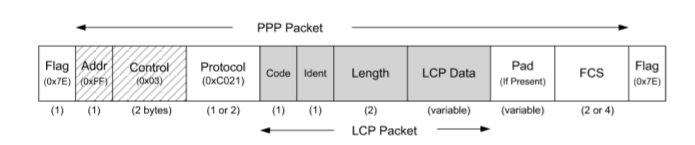
\includegraphics[width=500pt]{aufbau_ppp_frame}
  \end{center}
  \caption{Aufbau eines PPP-Frames}\cite{tcpipillustrated}
  \label{abb:aufbau_ppp_frame}
 \end{figure}

Diverse oben genannte Felder können in ihrer Länge variieren, da 
diese während des Verbindungsaufbaus vom \ac{LCP} ausgehandelt werden.

\paragraph{LCP Frame} Um die effizienteste Verbindungsart zu finden, benutzen PPP-Systeme
immer \ac{LCP} um die korrekten Parameter auszuhandeln. LCP-Nachrichten in ausgetauschten
PPP-Frames enthalten somit alle Konfigurationsoptionen für die sich gerade aufbauende
Verbindung. Ist eine Konfiguration gefunden, die beide Knoten unterstützen folgt der
Link-Establishment-Prozess. Ist dieser erreicht müssen danach keine weiteren redundanten
Paketinformationen im Header mitgetragen werden.

Ein LCP-Frame ist wie folgt aufgebaut:
\begin{itemize}
	\item code (1 Byte) - hexadezimal - enhält den Messagetyp (als Codes spezifiziert)
	\item identifier (1 Byte) - hexadezimal - mit diesen werden Anfragen bzw. Antworten mit einzelnen LCP-Transaktionen in Verbindung gebracht
	\item length (2 Byte) - hexadezimal - beinhaltet die Länge der Nachricht (inklusive code, identifier, length, data)
	\item data (variabel) - hexadezimal - Nutzdaten
\end{itemize}

\ac{LCP} ist so entworfen, dass Hersteller ihre eigenen Optionen einsetzen können, ohne
selbige explizit über \ac{IANA} spezifizieren zu müssen. Dokumentiert ist dies in \textbf{RFC2153}.

\paragraph{Aufbauphasen} Nachfolgend werden die verschiedenen Aufbauphasen des
PPP-Protokolls erläutert. Im \Anhang{abb:aufbauphasen_pppverbindung} befindet
sich eine Abbildung, die diesen Vorgang illustriert.

\textbf{Link Dead Phase:}
Beide Systeme fangen mit dieser Phase an und enden hiermit wieder.
Grundlage ist, dass außer (maximal) dem Link auf physischer Ebene,
keine Verbindung zwischen beiden Endpunkten besteht. Normalerweise
wird nach sicherstellen des physischen Links von einer Seite der
Aufbau der Verbindung initiiert. Dies geschieht meist mit einer Form von Modem.
Nach Abschluss der Initiierung beginnt die nachfolgende Phase.

\textbf{Link Establishment Phase:}
Das initiierende System System sendet eine \ac{LCP}-Nachricht an das Zielsystem,
um Optionen anzufordern, die gesetzt werden sollen. Dazu gehören
Netzwerklayer-Protokoll, Authentifizierungsmethode und andere optionale
Funktionen. Sofern das Zielsystem alle angeforderten Optionen beherrscht,
kann dieses eine Bestätigung (\textbf{ACK}) an das Quellsystem senden.
Ist dies nicht der Fall, wird eine Anwort verfasst, die sowohl alle
\textit{nicht unterstützten} als auch alle \text{unterstützten} Optionen
enthält, damit das Quellsystem nach Empfang dieser Information eine
Verbindung initiieren kann, die in jedem Fall von beiden Seiten unterstützt
wird. Das erfolgreiche Abschließen dieser Phase führt zur nächsten Phase.

\textbf{Authentication Phase:}
Diese Phase ist optional. Ausgelöst wird sie durch das vorhandensein einer
Authentifizierungsoption in der LCP-Konfigurationsnachricht.
Zur Auswahl stehen z.B. \ac{PAP} oder \ac{CHAP}.
Hierbei greift PAP auf Username und Passwort, CHAP auf eines komplexeren Informationsaustausch
mit einem Challenge-Response-Verfahren zurück. Wobei der Erfolg immer zu nächsten
Phase führt ist die Reaktion bei Misserfolg des Vorgangs Protokollabhängig.

\textbf{Link Quality Monitoring:}
Diese Phase ist wie ihr Vorgänger ebenfalls optional - ebenfalls ausgelöst durch
die gewählt Option in der LCP-Nachricht.
Hier aus mehreren Protokollen gewählt werden. Eines davon ist standardisiert:
das 'Link Quality Report Protocol'. Registriert werden unter anderem der Linktraffic
sowie Fehlermeldungen.

\textbf{Network Layer Protocol Configuration:}
Wie bereits erwähnt unterstützt PPP  das multiplexen von Protokollen auf
Netzwerklayerebene. Für jedes einzelne, das eingesetzt wird,
führt das System einen separaten Prozess des Verbindungsaufbaus durch.
Jedes Netzwerklayerprotokoll verfügt über einen eigenes \ac{NCP} sowie \ac{IPCP}.
Vergleichbar ist dies mit dem Aufbau von \ac{LCP} - nur spezifischer.

\textbf{Link Open Phase:}
Nachdem alle individuellen Optionen und NCP-Exchanges erfolgreich durchgeführt wurden,
ist der Verbindungsaufbau komplett und Protokolldaten können jetzt über den aufgebauten
Link in beide Richtungen ausgetauscht werden.

\textbf{Link Termination Phase:}
Wird die Verbindung absichtlich (Ablauf der Session, Authentifizierungsfehler)
oder durch Fehler o.ä. physikalisch getrennt, wird im Regelfall über \ac{LCP}
eine 'Terminate Request Message' versandt. Diese kann von der Gegenseite
angenommen (\textit{AKC}) werden, sofern die grundlegende Verbindung noch aktiv ist.
Beide Systeme sind dann wieder in der ursprünglich genannten 'Link Dead Phase'.
Eine Terminierung der Verbindung ist neben \ac{LCP} auch auf \ac{NCP}-Ebene möglich,
damit die PPP-Verbindung trotz 'Terminierung' bestehen bleibt.


\subsubsection{Architektur PPPoE}
Zur Realisierung der Verbindung zwischen Authentifizierungsstelle und
Endgerät wurde aufgrund der Beschaffenheit des Raspberry Pis eine
Ethernetverbindung gewählt. Dieser wird das im vorangegangenen
Abschnitt erläuterte \ac{PPP}-Protokoll zugrunde gelegt.
In Ethernetframes werden PPP-Daten als Nutzdaten enkapsuliert.
Diese Methode wurde auch im realen Umfeld dazu entwickelt \ac{ISP}s die
Möglichkeit zu geben Verbindungen über Kabelmodem oder DSL in Form
von Bridged-Topologien zu realisieren. Provider bewerkstelligen
so auch die Endpunktidentifikation, Accounting und Rechnungserstellung.
(Beschrieben wird der Standard in RFC2516)

\paragraph{Aufbauphasen}
im Kontext einer PPPoE-Verbindung sind Discovery und Session.
Beide werden nachfolgend erläutert.

\paragraph{Discovery}
ist die Phase, in der der Client PPPoE-Frames dazu verwendet einen
Zugangspunkt zu finden.

Dies geschieht in den folgenden Schritten bzw. Frames:
\begin{enumerate}
\item PPPoE Active Discovery Initiation (PADI) - Ein Frame, vom Client
      gesendet an die Broadcastadresse 0xFF-FF-FF-FF-FF-FF.
      Falls vorhanden, werden weitere Parameter als Payload 
      mitgeschickt. (Codefeld:9; Session-ID:0)
\item PPPoE Active Discovery Offer (PADO) - Ein Frame, der von der
      Authentifizierungsstelle an die Unicast MAC-Adresse des
      initiierenden Client geschickt wird. Weitere Parameter wie
      Service-Name o.ä. können ebenfalls mitgeschickt
      werden. (Codefeld:7; Session-ID:0)
\item PPPoE Active Discovery Request (PADR) - Ein Frame, der vom Client
      an die Unicat MAC-Adresse der Authentifizierungsstelle geschickt
      wird. (Codefeld:25; Session-ID:0)
\item PPPoE Active Discovery Session-Confirmation (PADS) - Ein Frame,
      der von der Authentifizierungsstelle an die Unicast MAC-Adresse
      des Client geschickt wird. Er enthält alle ausgehandelten Daten
      mit der zugewiesenen Session-ID. (Codefeld:101; Session-ID:XX)
\item PPPoE Active Discovery Terminate (PADT) - Ein Frame,
      der von beiden Endpunkten geschickt werden kann. Er signalisiert
      die gewünschte Verbindungsterminierung des Absenders.
      (Codefeld:167)
\end{enumerate}

\paragraph{Session}
ist die Phase, in der die PPPoE-Verbindung bereits erfolgreich
aufgebaut ist und Daten ausgetauscht werden können.
Dieser Zustand ist erreicht, sobald die PPPoE-Discovery-Phase
erfolgreich abgeschlossen ist.

<PPP-Daten im Ethernet Frame Abb?>

\subsection{Raspberry Pi}

Die Hardwaregrundlage für das Endgerät bietet die Plattform eines Raspberry Pis, einem Kleincomputer.

\subsubsection{Raspberry Pi Foundation}
Entwickelt wird der Raspberry Pi von der Raspberry Pi Foundation\footnote{\url{https://www.raspberrypi.org}}
(registriert in Großbritannien). Ziel der Organisation ist es,
seit Veröffentlichung des ersten Modells, einen kostengünstigen
Computer vorrangig für Bildungszwecke zu entwerfen. Auf diesem
Weg soll sowohl Erwachsenen als auch Kindern der Zugang zum
Programmieren oder anderen wissenschaftlichen Anwendungsgebieten
erleichtert werden.

Bisher wurden seit der initialen Veröffentlichung im Februar 2012(\cite{rasppifoundweb})
drei Generationen in unterschiedlichen Ausführungen
entwickelt. Die Bezeichnung A(+) bzw. B(+) gibt jeweils Aufschluss
über die jeweilige Ausführung.

\subsubsection{Hardware Modell B}
Das eingesetzte Modell B der ersten Generation verfügt über folgende Hardwarekomponenten:
\begin{itemize}
\item CPU - 700 MHz Singlecore ARM1176JZF-S
\item RAM - 512 MB
\item Speicherslot - SDHC
\item Grafikprozessor - Broadcom VideoCore IV
\end{itemize}

\subsubsection{Betriebssystem}
Als Betriebssystem gibt es für den Raspberry Pi eine breite Auswahl.
Neben einer Vielzahl von Media-Center-Plattformen sind auch alle
Desktop- bzw. Server-Versionen gängiger Linux-Derivate verfügbar:
Arch Linux, Puppy Linux, Raspbian, openSUSE, Gentoo Linux, Ubuntu Mate,
CentOS, Slackware, ...

\paragraph{Raspbian}
Aufgrund hoher Stabilität und Verfügbarkeit aller benötigten Treiber
(u.a. dem SIM-Kartenleser) wurde die auf \textit{Debian GNU Linux}\footnote{\url{https://www.debian.org/}}
basierende Distribution \textit{Raspbian}\footnote{\url{https://www.raspbian.org/}} ausgewählt.
Es erbt somit alle Eigenschaftem vom übergeordneten Debianprojekt.
So auch den Paketmanager \textit{dpkg} mit ca. 35.000 vorkompilierten
Softwarepaketen - in einigen Fällen für den Betrieb mit dem
Raspberry Pi optimiert. Nicht vorpaketierte Software kann auf dem Raspberry
Pi durch vorhandensein einer Vielzahl von Libraries und Build-Tools
für die ARM-Architektur kompiliert werden.

Über den rein funktionalen Konsolenbetrieb hinaus, wird Raspbian standardmäßig mit den
Windowmanagern XFCE oder LXDE ausgeliefert.

Nachdem im Juni 2012(\cite{raspbianweb}) die erste
Version fertiggestellt wurde ist Raspbian nach wie vor aktiv
in Entwicklung. Momentan im stabilen Debian-Release \textit{Jessie}.
Selbiges wird auch zur Umsetzung des Endgerätes eingesetzt.
Die vorkompilierten Pakete stammen dementsprechend aus dem aktuellen
\textit{stable}-Zweig, der häufig vor allem im Umfeld des Serverbetriebes
anzutreffen ist. Die Ursache hierfür ist die Tatsache, dass das
Projekt Pakete erst nach einem langen Testprozess im \textit{unstable}-
sowie darauffolgenden \textit{testing-}Zweig für den \textit{stable}-Zweig
freigibt. Im Kontrast zu gängigen Desktop-Distributionen, die
im Vergleich zu Debian stärker auf Aktualität achten.

Neben den Zielen der Raspberry Pi Foundation verfolgt das Projekt
auch die Ziele des Debian/GNU-Projekts. Es ist dementsprechend unter
den \textit{Debian Free Software Guidelines}\footnote{\url{https://wiki.debian.org/DFSGLicenses}} lizensiert und durch die Raspbian-Community unabhängig
entwickelt.

\subsection{PC/SC}
Multitasking- und Multiuserbetrieb in modernen Betriebssystemen erfordert
auch das Bereitstellen eines Standards, um den Zugriff auf Chipkarten
dementsprechend zu organisieren. Ein Standard, der sich mit genau
dieser Problemstellung befasst ist der \textit{\ac{PC/SC}}-Standard.
Er abstrahiert die Kommunikation mit der Chipkarte so,
dass die Anwendung keine genaueren speziellen Informationen zur verwendeten
Karte benötigt. Lediglich die Kommunikation mit dem Standard
konformen Lesegerät muss durch den Treiber sichergestellt werden.

\subsubsection{Die PC/SC-Workgroup}
Entwickelt wurde PC/SC von verschiedenen Herstellern. Hauptsächlich
Gemalto, Microsoft, Infineon und Toshiba.

\subsubsection{Spezifikation und Aufbau der Schnittstelle}
Die Spezifikation definiert Schnittstellen, die dem Zugriff auf Chipkarten ausgehend
von mehreren Applikationen bzw. Nutzern ermgöglichen. Grundlegend
dafür benötigt werden neben dem Standardkonformen Treiber ein \ac{IFD} und
eine \textit{PC/SC}-konforme Chipkarte (\ac{ICC} nach ISO7816-1,2 und 3).

 \begin{figure}[htp]
  \begin{center}
   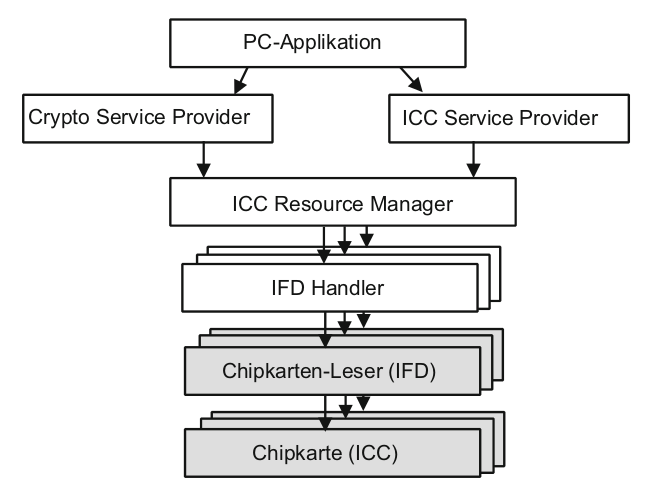
\includegraphics[width=300pt]{pcscspec_chipkartenitsicherheit}
  \end{center}
  \caption{Architektur des PC/SC-Standards}\cite{spitz11}
  \label{abb:architektur_pcsc}
 \end{figure}

Der Unterschied zum ähnlichen CT-API-Standard fängt in der Ebene
des \textit{ICC Resource Managers} an. Also der Abstraktion der
APDU-Schnittstelle in der Chipkartenmiddleware.\cite{spitz11}
Selbiger Manager organisiert sowohl die Vergabe von Terminals inklusive
der vorhandenen Chipkarte, als auch das Zuordnen zusammenhängender
APDU-Kommandoketten.

Losgelöst davon können Daten auf der Chipkarte abgelegt werden. Im Umfeld
der SIM-Karte sind dies Kontakte, SMS, o.ä. Hierfür zuständig ist der
\textit{ICC Service Provider}. Ebenfalls dazu gehören administrative Dateisystemzugriffe
wie das Ändern des PIN-Codes.

Der \textit{Cryptographic Service Provider} ist die ausführende Komponente
der auf der Chipkarte implementierten Algorithmen zur Authentifizierung mittels
Kryptoalgorithmen. Auslöser für die Aufteilung in zwei Schnittstellen -
\textit{Crypto Service Provider} und \textit{ICC Service Provider} sind
rechtliche Grundlagen. In manchen Staaten ist der Import von
Verschlüsselungtechnologien auf diesem Weg untersagt.

Unter Einhaltung des Standards ist es mit oben genannter Architektur möglich,
dass parallel aus verschiedenen Anwendungen auf unterschiedliche Konstellationen
von Chipkarten und Lesern zugegriffen wird.

Sowohl unter Windows als auch in vielen Linux-Distributionen sind
\textit{PC/SC-Treiber} mittlerweile verbreitet.

\subsubsection{PCSClite}
Die unter Linux-Distributionen verfügbare Version ist
PCSClite\footnote{\url{https://pcsclite.alioth.debian.org/}}.
Das von David Corcoran gestartete Projekt M.U.S.C.L.E
(Movement for the Use of Smart Cards in a Linux Environment)
wird mittlerweile hauptsächlich von Ludovic Rousseau
weitergeführt\cite{pcscliteweb}.

Neben diversen Linux-Distributionen werden auch Mac OSX und diverse
BSD- sowie Unix-Derivate unterstützt.

\subsection{Die Sprache Python}

\subsection{pysim}
Pysim\footnote{\url{https://github.com/kevinprince/pysim}} ist ein Tool,
welches Operationen direkt auf der SIM-Karte implementiert.
Sowohl Kryptoalgorithmen wie Milenage als auch administrative Dateisystemzugriffe
bis hin zur Verwaltung von Telefonbuch, SMS oder ähnlichem.
Unterstützt sind 3G und UMTS-Authentifizierungsvorgänge.

Pysim kennt verschiedene Modi und nimmt dementsprechend unterschiedliche
Parameter entgegen. Verfügbare Parameter sind Chipkartentyp, verwendetes
Device (im Betriebssystem /dev/ttyX) und Baudrate\cite{pysimprince}.

Über den normalen Betrieb einer SIM-Karte (also Authentifizierung, Auslesen, etc.)
ist es mit Pysim auch möglich Werte auf programmierbaren SIM-Karten zu setzen.

Neben abgeschlossenen Skripten ist auch die interaktive Nutzung auf der
python-Shell verwendbar.

\subsection{pyscard}
Zur Verwendung des Tools pysim wird zuerst eine Bibliothek benötigt,
die Smartcard-Support für Python bereitstellt. Diese Bibliothek
ist pysim. Sie fungiert als Schnittstelle zwischen dem Treiber \textit{PC/SC}
bzw. \textit{PCSClite} und der Python-Anwendung 
(dargestellt im \Anhang{abb:pyscard_schema}).

Implementierte Funktionen sind das Prüfen der gesteckten bzw. nicht gestecken
Chipkarte, der darauffolgende Verbindungsaufbau sowie das Versenden und
Empfangen von APDUs in hexadezimaler Darstellung.
Nach erfolgreichem Verbindungsaufbau kann somit eine Kommunikation via
APDUs stattfinden.

Veröffentlicht wurde pyscard als freie Software unter der
\textit{GNU Lesser General Public License}.


\subsection{Die Sprache C}

\subsection{Projektspecs}
